% EE/CS 148B HW3 — Vision-Language Models
% Writeup (typeset with pdflatex)
% ============================================================

\documentclass[11pt]{article}

\usepackage[margin=1in]{geometry}
\usepackage{amsmath, amssymb, amsthm}
\usepackage{graphicx}
\usepackage{hyperref}
\usepackage{bm}
\usepackage{enumitem}
\usepackage{float}
\usepackage{caption}
\usepackage{subcaption}
\usepackage{booktabs}
\usepackage{array}

\newcommand{\R}{\mathbb{R}}
\newcommand{\norm}[1]{\left\|#1\right\|}

\title{\textbf{EE/CS 148B --- Homework 3: Vision-Language Models}}
\date{Spring 2026}

\begin{document}
\maketitle

% ==============================================================
\section{Vision Transformer (\S2)}
% ==============================================================

\subsection*{Problem (vit\_pooling): CLS token vs.\ mean pooling}

For downstream tasks requiring spatial reasoning---counting objects, locating regions, or visual question answering that refers to specific image regions---\textbf{attention pooling} (or passing the full patch sequence) is expected to perform best. The CLS token aggregates global semantics into a single fixed-size vector, discarding which patch corresponds to which region of the image; mean pooling averages patch embeddings and preserves more distributed information but still loses the positional structure needed to answer relational questions (e.g., ``What color is the cube to the left of the sphere?''). Condensing the entire image to one vector before the language model means the LM has no access to spatial layout, making it impossible to localize objects or reason about their relative positions.

\subsection*{Problem (vit\_patch\_size): Effect of patch size}

\textbf{Number of patches for $224 \times 224$ images:}

\begin{center}
\begin{tabular}{ccc}
\toprule
Patch size $P$ & $N = (224/P)^2$ & Forward-pass time (ms) \\
\midrule
8  & 784 & $38.10 \pm 0.28$ \\
16 & 196 & $9.07 \pm 0.27$ \\
32 & 49  & $8.18 \pm 0.64$ \\
\bottomrule
\end{tabular}
\end{center}

Measurements taken on an A100-SXM4-80GB GPU, batch size 16, ViT with $d_{\mathrm{model}}=384$, 6 heads, 6 blocks. Averaged over 20 steps after 5 warmup steps using \texttt{torch.cuda.synchronize()}.

\paragraph{Discussion.}
Self-attention compute scales as $O(N^2 d_{\mathrm{model}})$, so shrinking $P$ from 16 to 8 quadruples $N$ (196$\to$784) and roughly 16$\times$ the attention compute. In practice, $P{=}8$ is ${\sim}4\times$ slower than $P{=}16$ on this hardware (38\,ms vs.\ 9\,ms). $P{=}16$ and $P{=}32$ are similarly fast because the bottleneck shifts to MLP and projection layers rather than attention at these sequence lengths.

\paragraph{When to accept the $P{=}8$ trade-off.}
When spatial fine-grained reasoning is critical (medical imaging, OCR, dense visual QA), the extra compute of small patches is justified because higher-resolution feature maps enable the model to distinguish subtle spatial patterns that coarser patches would merge.

% ==============================================================
\section{CLIP-Style Contrastive Pretraining (\S3)}
% ==============================================================

\subsection*{Problem (infonce): Symmetric InfoNCE}

The symmetric InfoNCE loss is
\[
\mathcal{L} = \tfrac{1}{2}\bigl(\mathrm{CE}(S, y) + \mathrm{CE}(S^\top, y)\bigr),
\quad S = \texttt{image\_embeds}\,\texttt{text\_embeds}^\top \cdot e^{\texttt{logit\_scale}}.
\]

\paragraph{Why symmetric.}
The first term $\mathrm{CE}(S, y)$ trains each image embedding to rank its paired caption above all other captions in the batch (image-to-text). The second term $\mathrm{CE}(S^\top, y)$ trains each text embedding to rank its paired image above all other images (text-to-image). Averaging both directions makes the shared embedding space isotropic with respect to both modalities and ensures both encoders receive equal gradient signal.

\subsection*{Problem (clip\_train): CLIP pretraining on EuroSAT}

\textbf{Hyperparameters:} \texttt{img\_size=64}, \texttt{patch\_size=8}, $d_{\mathrm{model}}=384$, 6 heads, 6 blocks, batch size 256, lr $=3\times10^{-4}$, AdamW (weight decay 0.1), cosine schedule with 200 warmup steps, 20 epochs.

\begin{figure}[H]
\centering
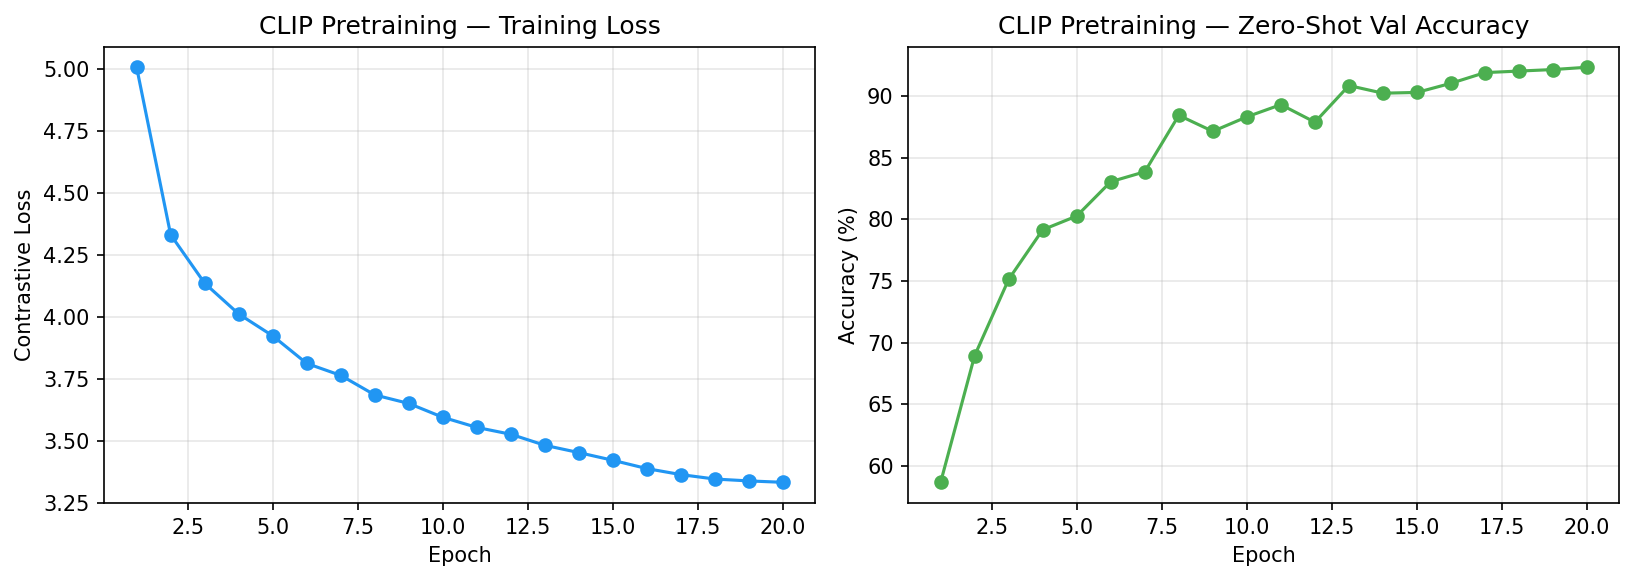
\includegraphics[width=0.9\textwidth]{clip_training_curves.png}
\caption{CLIP pretraining on EuroSAT: training contrastive loss (left) and zero-shot validation accuracy (right) vs.\ epoch.}
\end{figure}

\paragraph{Discussion.}
Training loss decreases steadily from 5.0 to 3.3 across 20 epochs, while zero-shot validation accuracy rises rapidly to ${\sim}88\%$ in the first 8 epochs and then gains more slowly, reaching 92.3\% at epoch 20. Training loss continues to improve even after validation accuracy plateaus above 90\%, because the loss measures fine-grained pairwise similarity across all batch pairs (many of which share the same class-prompt caption in EuroSAT), whereas accuracy only measures coarse class-level assignment.

\subsection*{Problem (clip\_zeroshot): Qualitative analysis}

\begin{figure}[H]
\centering
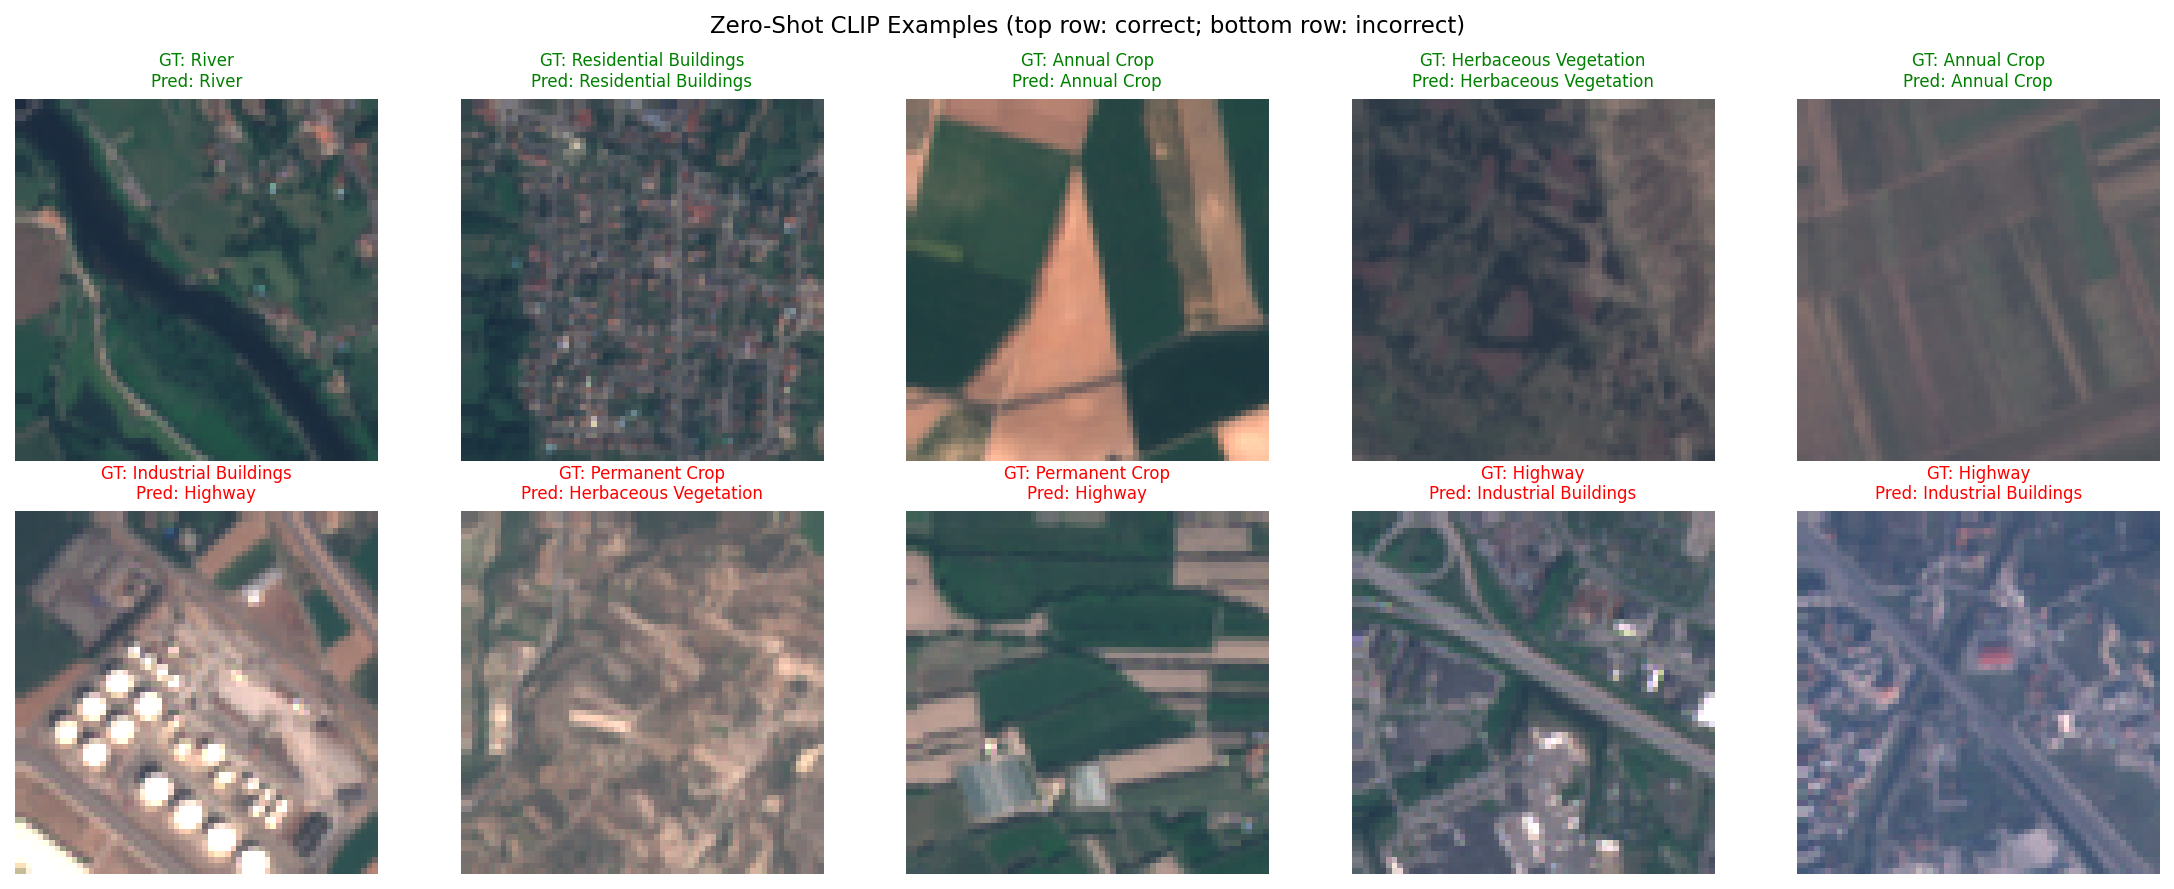
\includegraphics[width=\textwidth]{clip_zeroshot_examples.png}
\caption{Ten zero-shot CLIP classification examples on the EuroSAT test set (top row: correct, green titles; bottom row: incorrect, red titles). Ground-truth (GT) and predicted class labels are shown for each image.}
\end{figure}

Five correctly classified and five incorrectly classified test images are shown above. Correct classifications include \textit{River}, \textit{Residential Buildings}, \textit{Annual Crop}, and \textit{Herbaceous Vegetation} --- all visually distinctive at $64{\times}64$. Incorrect predictions show systematic confusions: \textit{Permanent Crop} is mistaken for \textit{Herbaceous Vegetation} (both appear as fine-textured green patches) and for \textit{Highway} (linear field boundaries resemble roads); \textit{Highway} is confused with \textit{Industrial Buildings} and vice versa (both show large grey paved areas from above). All mistakes involve visually similar categories, with no nonsensical errors observed.

This indicates the embedding space has learned meaningful semantic structure where nearby classes share visual appearance. Errors reflect genuine low-resolution ambiguity: at $64{\times}64$, fine texture differences between crop types and the grey-paved appearance shared by roads and industrial sites are not reliably distinguishable.

% ==============================================================
\section{LoRA Fine-Tuning (\S4)}
% ==============================================================

\subsection*{Problem (lora\_linear): LoRA-wrapped linear layer}

LoRA wraps an existing \texttt{nn.Linear} by freezing its weights and adding trainable low-rank matrices $A \in \R^{r \times d_{\mathrm{in}}}$ (Kaiming-uniform init) and $B \in \R^{d_{\mathrm{out}} \times r}$ (zero init). The forward pass computes
\[
W'x = Wx + \tfrac{\alpha}{r}\,BAx.
\]

\textbf{ViT with LoRA rank 8 parameter counts:}

\begin{center}
\begin{tabular}{lc}
\toprule
Metric & Value \\
\midrule
Total parameters     & 10{,}737{,}792 \\
Trainable parameters & 258{,}048 \\
Trainable ratio      & 2.40\% \\
\bottomrule
\end{tabular}
\end{center}

LoRA is applied to \texttt{q\_proj} and \texttt{v\_proj} in all 6 attention blocks (72 \texttt{LoRALinear} modules total).

\subsection*{Problem (lora\_compare): Full FT vs.\ LoRA vs.\ linear probe}

Starting from the CLIP-pretrained ViT, fine-tuned on RESISC45 for 10 epochs:

\begin{center}
\begin{tabular}{lcccc}
\toprule
Method & Test Acc & Trainable Params & Peak GPU Mem & Wall-clock \\
\midrule
Linear probe & 37.84\% & 17{,}325 & 239\,MB & 71\,s \\
LoRA ($r{=}8$) & 41.67\% & 275{,}373 & 1{,}177\,MB & 171\,s \\
Full FT & \textbf{63.54\%} & 10{,}755{,}117 & 1{,}719\,MB & 182\,s \\
\bottomrule
\end{tabular}
\end{center}

\paragraph{Discussion.}
Full fine-tuning achieves the best accuracy (63.5\%) by adapting all 10.7M parameters. The linear probe is extremely memory-efficient (17K params, 239\,MB peak) but lowest accuracy (37.8\%), indicating frozen CLIP features are not perfectly aligned with the 45-class RESISC45 distribution. LoRA sits in between: with only 2.4\% trainable parameters, it achieves 41.7\%---a 3.9\,pp improvement over the frozen probe at modest memory overhead. Full FT's 22\,pp advantage over LoRA likely stems from LoRA's rank constraint limiting how much feature representations can shift for 45 new classes.

\subsection*{Problem (lora\_rank): Rank sweep}

Sweep over ranks $r \in \{1, 2, 4, 8, 16, 32, 64\}$ with $\alpha = 2r$ (so $\alpha/r = 2$):

\begin{center}
\begin{tabular}{cccc}
\toprule
Rank $r$ & Test Acc & Trainable Params & Wall-clock \\
\midrule
1  & 33.00\% & 49{,}581 & 110\,s \\
2  & 35.71\% & 81{,}837 & 223\,s \\
4  & 39.44\% & 146{,}349 & 143\,s \\
8  & 41.67\% & 275{,}373 & 171\,s \\
16 & 44.41\% & 533{,}421 & 127\,s \\
32 & 46.86\% & 1{,}049{,}517 & 94\,s \\
64 & 50.98\% & 2{,}081{,}709 & 98\,s \\
\bottomrule
\end{tabular}
\end{center}

\paragraph{Discussion.}
Accuracy increases monotonically from $r{=}1$ (33.0\%) to $r{=}64$ (51.0\%) with no clear saturation point: gains per doubling remain roughly 2--4\,pp throughout the tested range, and the largest single jump (+4.1\,pp) actually occurs at $r{=}32 \to 64$. Even $r{=}64$ trails full fine-tuning (63.5\%) by 12.5\,pp, because for this small ViT ($d_{\mathrm{model}}{=}384$) the adapter is already $64/384 \approx 17\%$ of the feature dimension, far from the ``low-rank'' regime; in large-model fine-tuning the same rank represents $<2\%$ of the feature dimension, so LoRA converges faster relative to full FT. The near-linear trend on a log-rank axis suggests the fine-tuning update is not strongly low-rank for this task.

\begin{figure}[H]
\centering
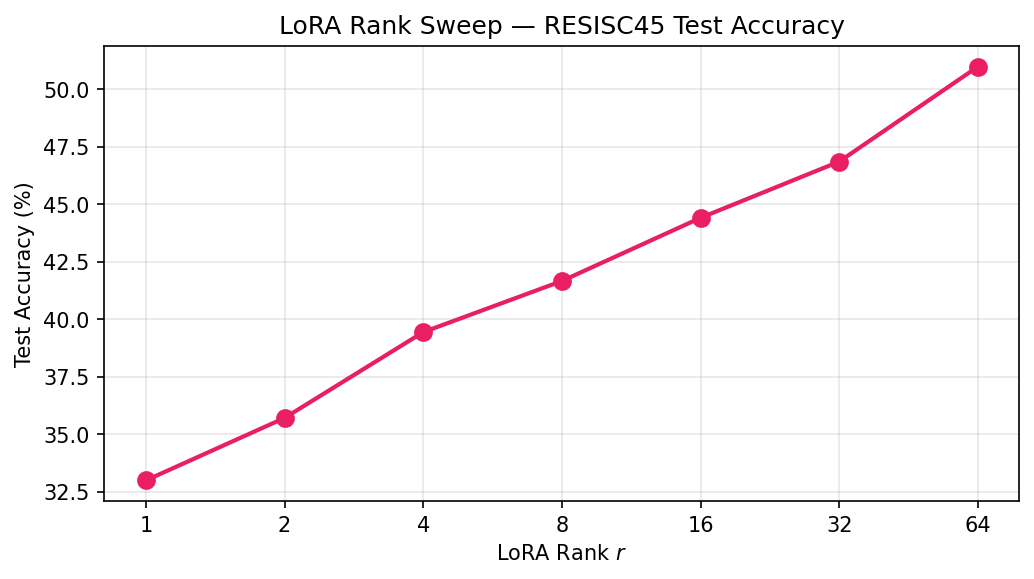
\includegraphics[width=0.6\textwidth]{lora_rank_sweep.png}
\caption{LoRA rank sweep on RESISC45: test accuracy vs.\ rank $r$ (log$_2$ scale).}
\end{figure}

% ==============================================================
\section{Vision-Language Model (\S5)}
% ==============================================================

\subsection*{Problem (projector): Vision-language projector}

The projector is a 2-layer MLP: \texttt{Linear}($d_{\mathrm{image}}$, $4 d_{\mathrm{image}}$) $\to$ GELU $\to$ \texttt{Linear}($4 d_{\mathrm{image}}$, $d_{\mathrm{decoder}}$).

\paragraph{Why more than a single linear layer.}
A single linear projection performs only an affine map between image and decoder embedding spaces, which may be insufficient when both the vision encoder and decoder are frozen. The nonlinear hidden layer lets the projector learn a richer, task-adaptive mapping---a ``translator'' that reshapes image features into the semantic geometry expected by the language model's embedding space. The $4\times$ hidden expansion adds capacity without a large parameter count.

\subsection*{Problem (masking): Image-block attention}

\paragraph{(1) Attention mask diagrams.}
For 4 visual tokens ($v_1,\ldots,v_4$) and 3 text tokens ($t_1,t_2,t_3$); $\blacksquare$ = attend, $\square$ = blocked.

\textbf{M1: Fully causal}
\begin{center}
\begin{tabular}{c|ccccccc}
 & $v_1$ & $v_2$ & $v_3$ & $v_4$ & $t_1$ & $t_2$ & $t_3$ \\
\hline
$v_1$ & $\blacksquare$ & $\square$ & $\square$ & $\square$ & $\square$ & $\square$ & $\square$ \\
$v_2$ & $\blacksquare$ & $\blacksquare$ & $\square$ & $\square$ & $\square$ & $\square$ & $\square$ \\
$v_3$ & $\blacksquare$ & $\blacksquare$ & $\blacksquare$ & $\square$ & $\square$ & $\square$ & $\square$ \\
$v_4$ & $\blacksquare$ & $\blacksquare$ & $\blacksquare$ & $\blacksquare$ & $\square$ & $\square$ & $\square$ \\
$t_1$ & $\blacksquare$ & $\blacksquare$ & $\blacksquare$ & $\blacksquare$ & $\blacksquare$ & $\square$ & $\square$ \\
$t_2$ & $\blacksquare$ & $\blacksquare$ & $\blacksquare$ & $\blacksquare$ & $\blacksquare$ & $\blacksquare$ & $\square$ \\
$t_3$ & $\blacksquare$ & $\blacksquare$ & $\blacksquare$ & $\blacksquare$ & $\blacksquare$ & $\blacksquare$ & $\blacksquare$ \\
\end{tabular}
\end{center}

\textbf{M2: Bidirectional inside image, causal elsewhere}
\begin{center}
\begin{tabular}{c|ccccccc}
 & $v_1$ & $v_2$ & $v_3$ & $v_4$ & $t_1$ & $t_2$ & $t_3$ \\
\hline
$v_1$--$v_4$ & \multicolumn{4}{c|}{full bidirectional block} & $\square$ & $\square$ & $\square$ \\
$t_1$ & $\blacksquare$ & $\blacksquare$ & $\blacksquare$ & $\blacksquare$ & $\blacksquare$ & $\square$ & $\square$ \\
$t_2$ & $\blacksquare$ & $\blacksquare$ & $\blacksquare$ & $\blacksquare$ & $\blacksquare$ & $\blacksquare$ & $\square$ \\
$t_3$ & $\blacksquare$ & $\blacksquare$ & $\blacksquare$ & $\blacksquare$ & $\blacksquare$ & $\blacksquare$ & $\blacksquare$ \\
\end{tabular}
\end{center}

\paragraph{(2) Expected performance.}
M2 (bidirectional inside image) should perform better because it aligns with how the ViT originally processed patches via bidirectional attention. Under M1, patch $v_i$ can only attend to $v_1,\ldots,v_{i-1}$, imposing an artificial left-to-right ordering on a 2D grid with no inherent sequential structure. M2 lets each visual token attend to all other visual tokens, preserving full image context.

\paragraph{(3) Experimental results} (500-step runs, all-patches injection):

\begin{center}
\begin{tabular}{lc}
\toprule
Mask mode & Val exact-match accuracy \\
\midrule
causal     & 34.8\% \\
image\_bidir & 30.8\% \\
\bottomrule
\end{tabular}
\end{center}

\paragraph{Discussion.}
Contrary to the theoretical expectation, \texttt{image\_bidir} (30.8\%) underperforms \texttt{causal} (34.8\%) at 500 steps. A likely explanation is that SmolLM2 was pretrained exclusively with causal attention; introducing a non-causal attention pattern for a block of tokens at the prefix disrupts the positional encoding assumptions baked into the pretrained weights. The model needs more steps to adapt to this novel masking regime, so the advantage of bidirectional image attention may only emerge with longer training or when the decoder is also fine-tuned.

\subsection*{Problem (injection\_compare): Which injection strategy is best?}

2000 training steps, freeze config A (projector only):

\begin{center}
\begin{tabular}{lcccc}
\toprule
Strategy & Val Acc & Visual Tokens & Peak GPU Mem & Time/step \\
\midrule
CLS only    & 37.0\% & 1  & 3{,}402\,MB & 77.2\,ms \\
All patches & \textbf{42.4\%} & 65 & 6{,}689\,MB & 74.1\,ms \\
Interleaved & 37.0\% & 65 & 6{,}689\,MB & 91.4\,ms \\
\bottomrule
\end{tabular}
\end{center}

\noindent\textit{Timing: freeze config A (projector only), batch size 4, averaged over 20 steps including backward pass.}

\paragraph{Discussion.}
All-patches injection (42.4\%) outperforms both CLS-only (37.0\%) and interleaved (37.0\%). CLS discards spatial information by pooling the entire image into one token. Interleaved injection, despite using all 65 visual tokens, performs the same as CLS-only here --- likely because the \texttt{<image>} placeholder is rare in the pretrained vocabulary and the model struggles to learn when to attend to interleaved visual tokens without fine-tuning the decoder. Direct prepending (all-patches) is the most natural format for a causal decoder seeing a prefix of visual tokens. Surprisingly, all-patches is slightly \emph{faster} than CLS-only per step (74 vs.\ 77\,ms) --- the 65-token prefix is long enough to saturate GPU memory bandwidth, masking the extra compute, while CLS incurs more Python/CUDA overhead per token. Interleaved is the slowest (91\,ms) due to the extra bookkeeping needed to splice visual tokens into arbitrary positions.

\subsection*{Problem (vlm\_qualitative): What has your VLM learned?}

Evaluated on 500 CLEVR-mini val examples with the best all-patches checkpoint (config A):

\begin{center}
\begin{tabular}{lc}
\toprule
Question type & Accuracy \\
\midrule
compare\_attr & 64.3\% \\
exist         & 58.3\% \\
spatial       & 43.6\% \\
overall       & 42.4\% \\
query\_attr   & 35.4\% \\
count         & 33.3\% \\
\bottomrule
\end{tabular}
\end{center}

The model handles yes/no questions best (\textit{exist}, \textit{compare\_attr}: $>58\%$) because these require only a binary decision about global scene properties. \textit{Count} questions are hardest (33.3\%): counting objects in a 64$\times$64 image requires precise spatial localization, which is challenging when the projector is the only trainable component. Example predictions:

\begin{center}
\begin{tabular}{p{8cm}ccc}
\toprule
Question (truncated) & Gold & Pred & \\
\midrule
Are there fewer gray metal cylinders...? & yes & yes & \checkmark \\
What number of things are left of...?    & 1   & 1   & \checkmark \\
What material is the red object?         & rubber & rubber & \checkmark \\
Is there anything else the same size as the brown thing? & yes & yes & \checkmark \\
Is the large matte cylinder the same color as the shiny cube? & no & no & \checkmark \\
How many things are either metal objects in front of the large purple cylinder or purple cylinders left of the brown thing? & 4 & 1 & $\times$ \\
Is there anything else that is the same shape as the small red shiny object? & no & yes & $\times$ \\
The metallic cylinder same size as the yellow sphere is what color? & purple & brown & $\times$ \\
What color is the tiny sphere? & cyan & brown & $\times$ \\
Does the blue rubber object have the same shape as the big metallic thing right of the matte cube? & no & yes & $\times$ \\
\bottomrule
\end{tabular}
\end{center}

\paragraph{Discussion.}
The model handles binary questions (\textit{exist}, \textit{compare\_attr}) best because the decoder can exploit language priors (defaulting to ``yes'' or a common attribute) with only a coarse visual signal. Counting errors (e.g., gold=4, pred=1) and color-attribute errors (e.g., gold=cyan/purple, pred=brown) are most likely \emph{encoder} failures: at $64{\times}64$ with 65 patch tokens, fine-grained spatial relations and small-object colors are poorly resolved, so increasing the image resolution or patch granularity should help. Incorrect exist answers (e.g., gold=no, pred=yes) are more likely \emph{decoder} failures driven by language priors, since the pretrained LM is biased toward ``yes'' for existence questions. To distinguish the two, one can run the same question through the text-only decoder (without any image): if it predicts the wrong answer, the fault is the language prior; if it is correct only when the image is provided, the fault is the encoder's inability to encode the relevant visual detail.

\subsection*{Problem (freezing): What to train, and when}

\begin{center}
\begin{tabular}{ccccccc}
\toprule
Config & Encoder & Projector & Decoder & Val Acc & Train Params & Peak Mem \\
\midrule
A & frozen  & trained & frozen       & 42.4\% & 2{,}067K   & 6{,}689\,MB \\
B & frozen  & trained & LoRA $r{=}8$ & 39.4\% & 2{,}886K   & 6{,}975\,MB \\
C & frozen  & trained & full FT      & 40.4\% & 363{,}888K & 10{,}276\,MB \\
D & full FT & trained & full FT      & \textbf{42.4\%} & 374{,}626K & 10{,}753\,MB \\
\bottomrule
\end{tabular}
\end{center}

\paragraph{Discussion.}
Config A (projector-only training) achieves 42.4\% at minimal cost---just 2M trainable parameters and ${\sim}6.7$\,GB peak memory---suggesting the frozen CLIP encoder already produces rich visual features that the projector can bridge to the decoder with only 2{,}000 steps.
Config B (decoder LoRA) performs \emph{worse} than A (39.4\% vs.\ 42.4\%), likely because adding LoRA adapters to a bfloat16 decoder introduces dtype and gradient-flow noise that destabilizes training without long enough fine-tuning to overcome the frozen pretrained decoder's priors.
Config C (full decoder FT) achieves 40.4\%, marginally below A: fully fine-tuning 363M decoder parameters on this small CLEVR dataset quickly overfits or shifts the decoder's language priors away from what the projector produces, hurting performance within 2{,}000 steps.
Config D (everything unfrozen) matches A at 42.4\% but with $181\times$ more trainable parameters and ${\sim}60\%$ more memory---the gains from end-to-end training cancel with overfitting at this step budget.
The consistent message is that for small step budgets on small datasets, training only the projector is surprisingly competitive: the frozen CLIP encoder and pretrained LM provide strong inductive biases that do not need to be overwritten.

% ==============================================================
\section{Positional Encodings and RoPE (\S6)}
% ==============================================================

\subsection*{Problem (rope\_1d): 1D RoPE --- norm preservation}

RoPE applies a rotation to each pair $(x_{2i}, x_{2i+1})$, an orthogonal transformation (rotation matrices have determinant 1 and preserve norms). Measured norm difference after applying RoPE:
\[
\max \left|\norm{x} - \norm{\mathrm{RoPE}(x)}\right| = 9.54 \times 10^{-7},
\]
confirming norm preservation up to floating-point precision.

\subsection*{Problem (rope\_vs\_learned): RoPE vs.\ learned positional embeddings}

\paragraph{Implementation.}
The ViT now supports three positional encoding modes via a \texttt{pos\_enc} argument:
\begin{itemize}
  \item \textbf{Learned PE} (default): a learnable $(1, N{+}1, d_{\mathrm{model}})$ embedding added to the input.
  \item \textbf{RoPE-1D}: no learned PE; instead, RoPE is applied to Q and K inside each attention head. CLS receives position 0; patch $i$ receives position $i{+}1$ in raster-scan order.
  \item \textbf{RoPE-2D}: the head dimension is split in half; the first half is rotated by the patch column index, the second by the row index. CLS receives $(0, 0)$.
\end{itemize}
For extrapolation, the ViT is trained at $64{\times}64$ (patch size 8, $8{\times}8 = 64$ patches) and evaluated zero-shot at $96{\times}96$ ($12{\times}12 = 144$ patches). Learned PE uses bilinear interpolation of the $8{\times}8$ embedding grid to $12{\times}12$; RoPE methods generalise naturally since frequencies are computed on-the-fly.

\paragraph{Results.}

\begin{center}
\begin{tabular}{lccc}
\toprule
PE method & Val acc ($64{\times}64$) & Test acc (96$\times$96 extrap.) & $\Delta$ (extrap.\ drop) \\
\midrule
Learned (bilinear interp.) & 92.33\% & 81.70\% & $-$10.6\,pp \\
RoPE-1D                    & 91.09\% & 77.83\% & $-$13.3\,pp \\
RoPE-2D                    & \textbf{92.45\%} & \textbf{80.53\%} & $-$11.9\,pp \\
\bottomrule
\end{tabular}
\end{center}

\paragraph{Discussion.}
At the training resolution, all three methods perform similarly (${\sim}91$--$92\%$). On extrapolation to $96{\times}96$, learned PE with bilinear interpolation degrades the least ($-10.6$\,pp), likely because bilinear resizing of the training grid is well-calibrated after 20 epochs. RoPE-2D extrapolates better than RoPE-1D ($-11.9$ vs.\ $-13.3$\,pp): by encoding true $(x,y)$ patch coordinates, 2D RoPE places the new $12{\times}12$ patches in a consistent spatial space, whereas 1D raster positions do not scale gracefully to a wider grid. Overall, RoPE does not clearly outperform learned PE for extrapolation in this setting, but 2D coordinates are a more principled inductive bias for image data.

\subsection*{Problem (rope\_2d): 2D RoPE}

\paragraph{Implementation.}
\texttt{RoPE2D} (in \texttt{basics/rope.py}) splits \texttt{head\_dim} into two halves. The first half applies 1D RoPE using the patch column index; the second applies 1D RoPE using the row index. This is equivalent to independent rotations along $x$ and $y$ axes so that the attention dot product encodes the 2D \emph{relative offset} $(\Delta x, \Delta y)$ between any two patches. The ViT is modified so that when \texttt{pos\_enc="rope2d"}, learnable PE is removed and all attention blocks use \texttt{RoPE2D} via custom \texttt{\_RoPEBlock} layers.

Zero-shot accuracy on EuroSAT (64$\times$64 training): \textbf{92.45\%}; extrapolation at 96$\times$96: \textbf{80.53\%}.

RoPE-2D matches learned PE in in-distribution accuracy and drops only 1.9\,pp more on extrapolation. Because 2D RoPE encodes the correct spatial relationship between patches (column-row coordinates) rather than an arbitrary raster order, it provides a more principled representation for image data where the 2D arrangement of features is semantically meaningful.

\subsection*{Problem (mrope\_written): Reasoning about M-RoPE}

\paragraph{(1) Naive 1D positions for 64 patch tokens + CLS + 50 text tokens.}
With 64 patch tokens plus 1 CLS token prepended before a 50-token text prompt, text tokens receive position IDs 65--114. SmolLM2 handles sequences of hundreds or thousands of tokens, so out-of-distribution positions are not the primary concern at this scale. However, 2D structure is completely lost: the 64 patch tokens get sequential 1D positions (0--63) encoding raster-scan order through an 8$\times$8 grid, but the model receives no $(x,y)$ coordinates, preventing reasoning about spatial relationships like ``the patch above'' or ``to the left.''

\paragraph{(2) First text token position under M-RoPE.}
The first text token receives position $(t{=}1,\, x{=}\texttt{grid\_size},\, y{=}\texttt{grid\_size})$, e.g.\ $(1,8,8)$ for an 8$\times$8 patch grid. This is sensible because: (a) $t{=}1$ marks the first text token ($t{=}0$ for all image patches), and (b) $x,y$ are set to $\max\_\mathrm{grid\_coord}+1$, so text spatial IDs do not overlap with image IDs. A 10-token prompt after a 64-patch image starts at spatial position $(8,8)$ rather than 64, staying closer to positions the pretrained LM expects.

\paragraph{(3) Why three dimension chunks $(t,x,y)$ rather than just $(x,y)$.}
M-RoPE splits the head dimension into three chunks for temporal, horizontal, and vertical coordinates. If only $(x,y)$ were used, text tokens would have no dedicated way to encode sequential ordering---all text tokens would share the same $(x,y)$ or encode order only in one spatial axis, confusing language modeling. The temporal $t$ chunk is critical because language is inherently sequential, while image patches have no temporal ordering. Splitting into three chunks lets each coordinate type apply to the right tokens without interference.

\end{document}
